\Needspace{4in}
\begin{prob}

    Suppose the Bellman-Ford algorithm is run on the following graph using node $a$ as the source node:

    \begin{center}
        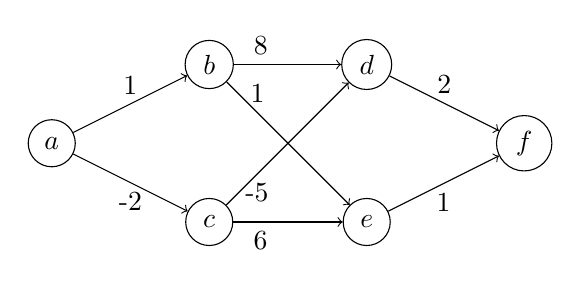
\begin{tikzpicture}
            {
                \tikzset{every node/.style = {shape=circle, draw, minimum size=17pt}}

                \node (a) at (0, 0) {$a$};
                \node (b) at (2, 1) {$b$};
                \node (c) at (2, -1) {$c$};
                \node (d) at (4, 1) {$d$};
                \node (e) at (4, -1) {$e$};
                \node (f) at (6, 0) {$f$};
            }

            % draw an edge with label in the middle
            \draw (a) edge[->] node[above, midway] {1} (b);
            \draw (a) edge[->] node[below, midway] {-2} (c);

            \draw (b) edge[->] node[above, near start] {8} (d);
            \draw (b) edge[->] node[above, near start] {1} (e);
            \draw (c) edge[->] node[below, near start] {-5} (d);
            \draw (c) edge[->] node[below, near start] {6} (e);

            \draw (d) edge[->] node[above, midway] {2} (f);
            \draw (e) edge[->] node[below, midway] {1} (f);

        \end{tikzpicture}
    \end{center}

    Suppose when \python{graph.edges} is called, the edges are returned in the order:

    \begin{center}
        $
        (a, b),
        (c, e),
        (d, f),
        (c, d),
        (b, d),
        (b, e),
        (a, c),
        (e, f)
        $
    \end{center}

    After one iteration of the outer loop of Bellman-Ford, what is the
    estimated distance to node $d$?

    \inlineresponsebox[.75in]{9}


\end{prob}
